
\begin{frame}{Recap \& Refresh}

	If there is no closed form for the posterior distribution:
        \begin{itemize}
                \item asymptotic methods (e.g. Normal approximation)
		\item direct sampling (Monte Carlo)
		\item non-iterative sampling (e.g. rejection algorithm)
		\item iterative sampling: MCMC (Gibbs vs. Metropolis algorithms)
        \end{itemize}

\end{frame}

\section{Approximate Bayesian Computation}

\begin{frame}{Intended Learning Outcomes}

        At the end of this day you will be able to:
        \begin{itemize}
                \item appreciate the applicability of ABC,
		\item describe the rejection algorithm,
		\item critically discuss the choice of summary statistics,
                \item implement ABC methods in \texttt{R}.
        \end{itemize}

\end{frame}

\begin{frame}{Posterior probability distribution}

	\begin{equation*}
        	p(\theta|x) = \frac{p(x|\theta)\pi(\theta)}{p(x)}
  	\end{equation*}
    	which can be difficult as the marginal likelihood
       	\begin{equation*}
		p(x) = \int p(x|\theta) \pi(\theta) d\theta
       	\end{equation*}
    	might involve a high dimensional integral difficult (or impossible) to solve.
               
\end{frame}

\begin{frame}{Sampling from the posterior}

	\begin{itemize}
		\item If the likelihood can be evaluated up to a normalising constant, Monte Carlo 
		methods can be used to sample from the posterior.
		\item If the likelihood function becomes difficult to define and compute, it is 
		easier to \textit{simulate} data samples from the model given the value of a parameter.
	\end{itemize}

\end{frame}

\frame{
\frametitle{Rejection algorithm}

	If data points are \textbf{discrete} and of low dimensionality, given observation $y$, 
	repeat the following until $N$ points have been accepted:
        \begin{enumerate}
        	\item Draw $\theta_i \sim \pi(\theta)$
        	\item Simulate $x_i \sim p(x|\theta_i)$
        	\item Reject $\theta_i$ if $x_i \neq y$ 
        \end{enumerate}
        These are sampled from $p(\theta|x)$.

}

\frame{
\frametitle{Rejection algorithm (elephants are back!)}

	Example:\\
	\begin{itemize}
		\item We observe $4$ herds arriving.
		\item The likelihood is Poisson-distributed and the prior is Gamma-shaped $G(3,1)$.
		\item The posterior distribution is Gamma distributed with shape parameter 
		$3+4=7$ and scale/rate $0.5$.
	\end{itemize}

	Let's assume that we can't evaluate the likelihood but we know how to \textit{simulate} $y$ 
	given a certain value of our parameter $\theta$.

	Exercise:\\
	Calculate the posterior distribution of $\theta$ in \texttt{R}.

}

\frame{
\frametitle{Rejection algorithm}

	If data points are \textbf{continuous} and of low dimensionality, given observation $y$, 
	repeat the following until $N$ points have been accepted:
        \begin{enumerate}
        	\item Draw $\theta_i \sim \pi(\theta)$
        	\item Simulate $x_i \sim p(x|\theta_i)$
        	\item Reject $\theta_i$ if $\rho(x_i,y) > \epsilon$        
        \end{enumerate}
        where $\rho(\cdot)$ is a function measuring the distance between simulated and observed points.

}

\frame{
\frametitle{Rejection algorithm (hot water is back!)}

	Example (water temperature):\\
	\begin{itemize}
		\item $\theta$ is continuous with prior distribution $U(80.1,110.3)$.
		\item we have a single observation $y=91.3514$.
		\item as $\rho(\cdot)$ we use the Euclidean distance:
        	\begin{equation}
        		\rho(x_i, y) = \sqrt[]{(x_i-y)^2}
        	\end{equation}
	\end{itemize}

        We can't evaluate the likelihood function but we can simulate observations 
	that are distributed according to it.
        
	Exercise:\\
	Calculate the posterior distribution of $\theta$ using \texttt{R}.
}

\frame{
\frametitle{Rejection algorithm v2}

	Alternatively, $\epsilon$ is the proportion of accepted simulations 
	(ranked by distance with observations).
	In this case one sets the number of simulations to be performed 
	(not the number of accepted simulations).

}

\frame{
\frametitle{Rejection algorithm v2}

	Exercise (water temperature):
	\begin{enumerate}
        	\item $Y=\{91.34, 89.21, 88.98\}$
        	\item $\theta$ has prior $N(\mu=90,\sigma^2=20)$ for $80 \geq \theta \leq 110$
        	\item the simulating function is \texttt{simulate <- function(param) rnorm(n=1, 
		mean=param, sd=sqrt(10))}
        	\item the distance function is $\rho(x_i, Y)=\frac{\sum_{j \in Y} 
		\sqrt[]{(x_i-j)^2}}{|Y|}$
        	\item $N=10,000$ and $\epsilon=0.05$
	\end{enumerate}
        
        Tasks:
        \begin{enumerate}
        \item plot the sampled prior distribution
        \item plot the distribution of ranked distances with indication of 5\% threshold
        \item plot the posterior distribution
	\item calculate notable quantiles and HPD 95\%
        \end{enumerate}
        
}

\frame{
\frametitle{Rejection algorithm with high dimensionality}

	If data points are of \textbf{high dimensionality}, given observation $y$, 
	repeat the following until $N$ points have been accepted:
        \begin{enumerate}
        	\item Draw $\theta_i \sim \pi(\theta)$
        	\item Simulate $x_i \sim p(x|\theta_i)$
        	\item Reject $\theta_i$ if $\rho(S(x_i),S(y))>\epsilon$
        \end{enumerate}
        with $S(y)$ being summary statistics.

}

\frame{
\frametitle{Rejection algorithm}

 \begin{figure}[!ht]
        \centering
		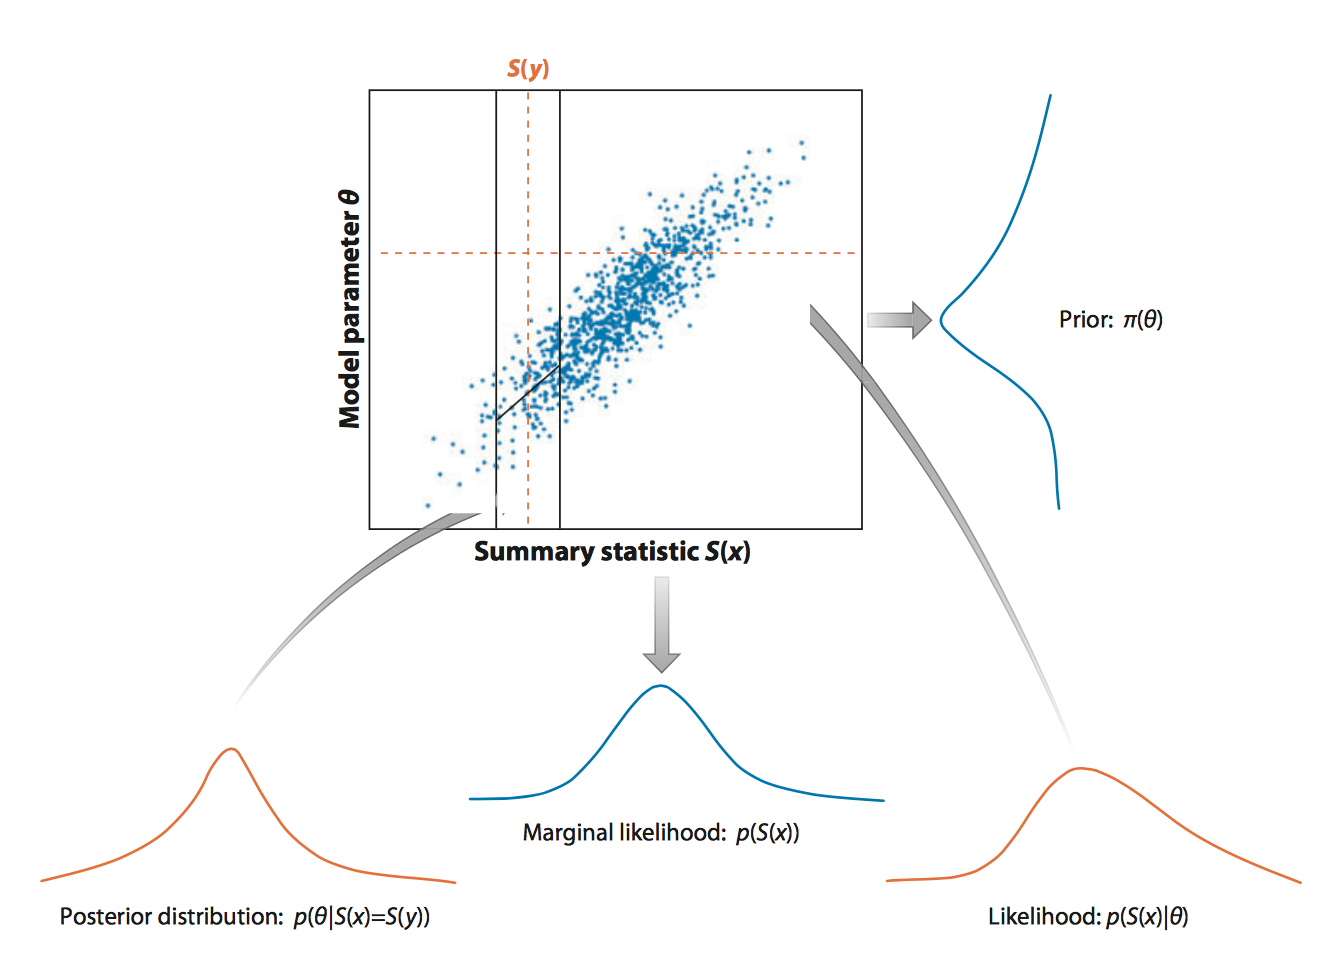
\includegraphics[width=6cm]{Images/ABC.png}
        \caption{From Beaumont 2010 Annu Rev Ecol Evol Syst. Rejection- and regression-based approximate Bayesian computation (ABC).}
       	\label{Fig:ABC}
		\end{figure}

}

\frame{
\frametitle{Summary statistics}

	\begin{itemize}
		\item The choice of summary statistics is a mapping from a high dimension 
		to a low dimension.
		\item Some information is lost, but with enough summary statistics much of 
		the information is kept.
		\item The aim for the summary statistics is to satisfy the Bayes' sufficiency:
        \begin{equation*}
        p(\theta|x)=p(\theta|S(x))
        \end{equation*}
\end{itemize}

	Issues?

	\pause
	Solutions:
	\begin{enumerate}
		\item use a wider acceptance tolerance
		\item perform a better sampling from the prior
	\end{enumerate}
        
}

\frame{
\frametitle{Regression-based ABC}

\small
\begin{enumerate}
		\item Given observation $y$ repeat the following until $M$ points have been generated:
		A. Draw $\theta_i \sim \pi(\theta)$;
        B. Simulate $x_i \sim p(x|\theta_i)$
        \item Calculate $S_j(x)$ for all $j$ and $k_j$
        \item $\rho(S(x),S(y)):\sqrt[]{\sum_{j=1}^s ( \frac{S_j(x)}{k_j} - \frac{S_j(y)}{k_j} )^2 }$
        \item Choose $\epsilon$ such that the proportion of accepted points $P_\epsilon=\frac{N}{M}$
        \item Weight the simulated points $S(x_i)$ using $K_\epsilon(\rho(S(x_i),S(y)))$ 
 		\begin{equation*}
        \begin{displaystyle}
  		K_\epsilon(t) = 
  		\begin{cases}
    	\epsilon^{-1}(1-(t/\epsilon)^2) & \text{for } t \leq \epsilon \\
		0 & \text{for } t > \epsilon 
        \end{cases}
		\end{displaystyle}
        \end{equation*}       
        \item Apply weighted linear regression to the $N$ points that have nonzero weight to obtain an estimate of $\hat{E}(\theta|S(x))$
        \item Adjust $\theta_i^*=\theta_i-\hat{E}(\theta|S(x))+\hat{E}(\theta|S(y))$
	\tiny
        \item The $\theta_i^*$ with weights $K_\epsilon(\rho(S(x_i),S(y)))$ are random draws from an approximation of $p(\theta|y)$.
         \end{enumerate}

}

\frame{
\frametitle{MCMC-ABC}

Initialise by sampling $\theta^{(0)} \sim \pi(\theta)$.\\
        At iteration $t \geq 1,$
        \begin{enumerate}
        \item Simulate $\theta' \sim K(\theta|\theta^{(t-1)})$ where $K(\cdot)$ is a proposal distribution that depends on the current value of $\theta$
        \item Simulate $x \sim p(x|\theta')$.
        \item If $\rho(S(x),S(y))<\epsilon$ (rejection step),
        \begin{itemize}
        \item $u \sim U(0,1),$
        \item if $u \leq \pi(\theta')/\pi(\theta^{(t-1)}) \times K(\theta^{(t-1)}|\theta')/K(\theta'|\theta^{(t-1)})$,\\
        update $\theta{(t)}=\theta'$;
        \item otherwise\\
        $\theta{(t)}=\theta^{(t-1)}$;
        \end{itemize}
        \item otherwise $\theta{(t)}=\theta^{(t-1)}$.
        \end{enumerate}

}

\frame{
\frametitle{Model assessment}

\begin{block}{Model choice}
        Given a series of model $\mu_1, \mu_2, ..., \mu_N$ with prior probabilities $\sum_i \pi(\mu_i)=1$, it is of interest to calculate Bayes factors between two models $i$ and $j$:
        \begin{equation}
		\frac{p(\mu_i|x)}{p(\mu_j|x)} \div \frac{p(\mu_i)}{p(\mu_j)}  
        \end{equation}
\end{block}

}

\frame{
\frametitle{Choice of summary statistics}

The more the merrier?

  \begin{figure}[!ht]
        \centering
		
\includegraphics[width=5cm]{Images/LucyBlanket.jpg}
        \caption{Choosing summary statistics: the issue of pulling a short blanket.}
       	\label{Fig:LucyBlanket}
		\end{figure}
        
}

\frame{
\frametitle{Choice of summary statistics}

\begin{enumerate}
\item One could calculate the ratio of posterior density with or without a particular summary statistic.
        Departures greater than a threshold are suggestive that the excluded summary statistic is important.
\item Different summary statistics can be weighted differently according to their correlation with some model parameters.
\item The number of summary statistics can also be reduced via multivariate dimensional scaling
summary statistics should be scaled in order to have equal mean and variance, if normally distributed.
\item Even if there is no need of a strong theory relating summary statistics to model parameters, it is suitable to have some expectations.
\end{enumerate}


}

\frame{
\frametitle{Model validation}

Validation is the assessment of goodness-of-fit of the model and comparing alternative models, to distinguish errors due to the approximation from errors caused by the choice of the model.

\begin{enumerate}
\item The distributions of simulated summary statistics are visualised and compared to the corresponding target statistic.
        If the target is outside, then this could be a problem in the model.
\item The observations are compared with the posterior predictive distribution.
        This can be done by simulating data with parameters drawn randomly from the current posterior distribution.
\end{enumerate}

}

\frame{
\frametitle{Applications of ABC in biology}

Population genetics, agent-based models, protein interaction networks, speciation rates under a neutral ecological model, extinction rates from phylogenetic data, epidemiology, ...

\begin{figure}[!ht]
        \centering
		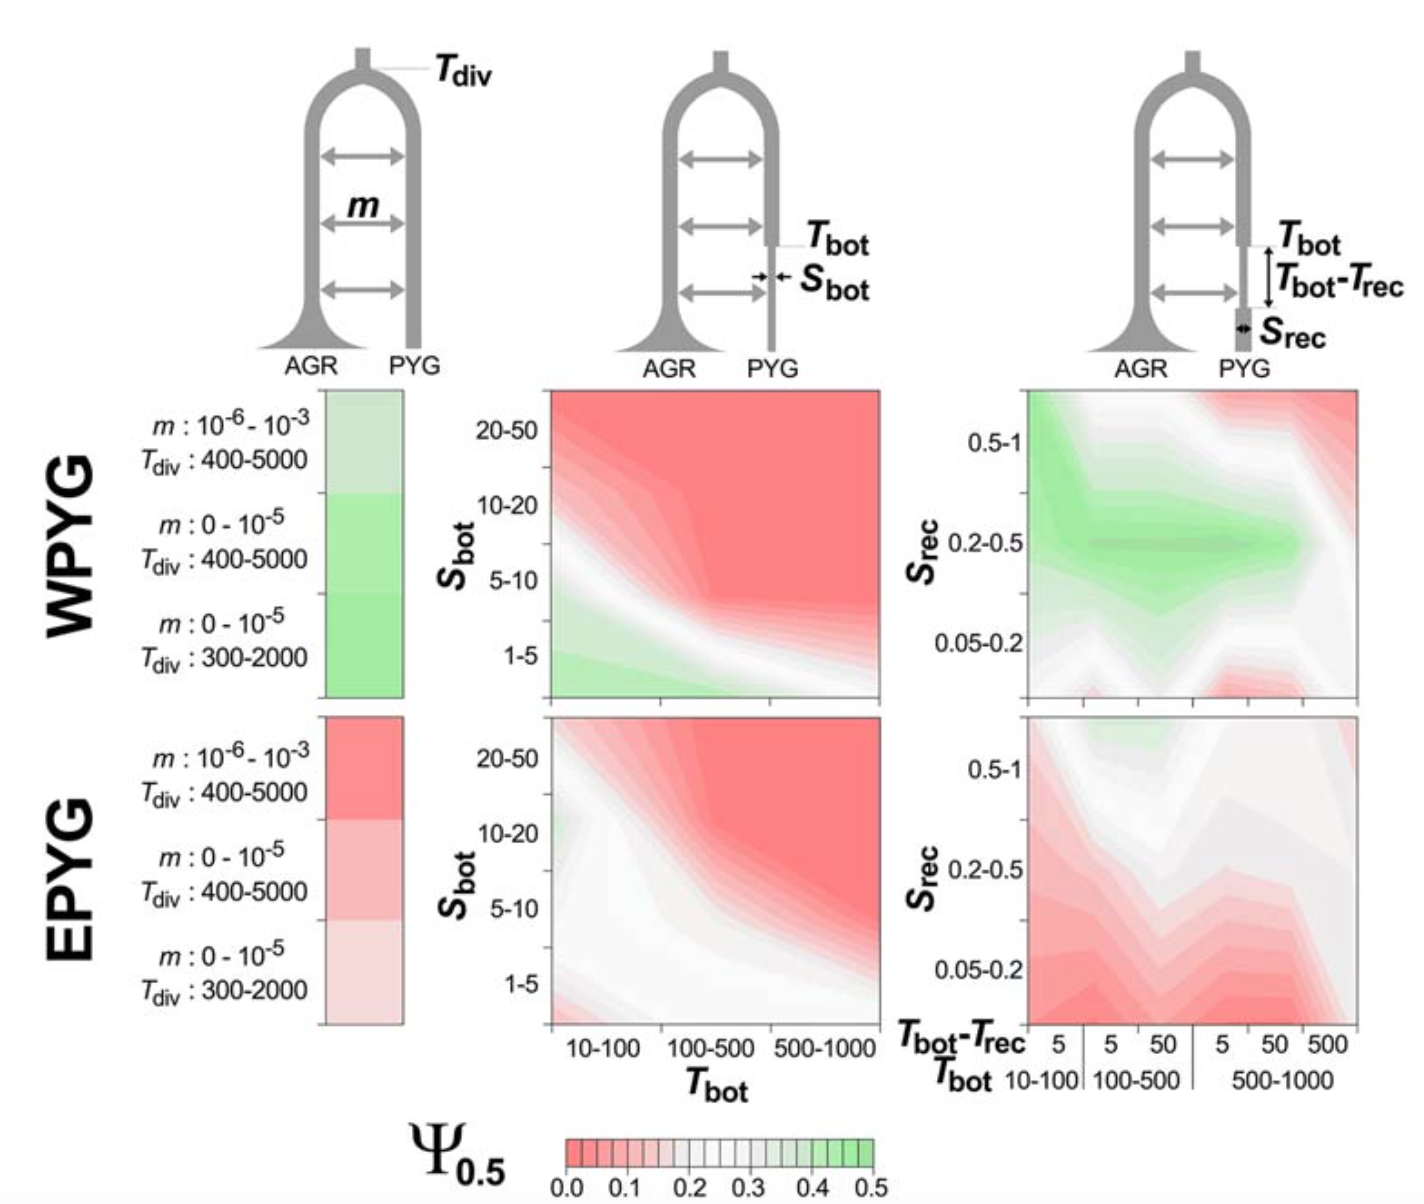
\includegraphics[width=3.5cm]{Images/Patin1.png}
        \caption{\tiny{Patin et al. (2009). Different models simulating the demographic regime of the African groups and the mean proportion of small distances ($\Omega_{0.5}$) obtained in comparisons with simulated statistics.}}
       	\label{Fig:Patin1}
		\end{figure}
        
}

\frame{
\frametitle{To ABC or not to ABC?}

\begin{itemize}
\item When a likelihood function is known and can be efficiently evaluated, then there is not advantage to use ABC.
\item When the likelihood function is known but difficult to evaluate in practise, the ABC is a valid option.
\item Many scenarios in evolutionary biology or ecology can be generated by simulations.
\item ABC can be useful for initial exploratory phase.
\item Be careful with the choice of your priors!
\end{itemize}

}





